\chapter{Future colliders}
aaa

\section{Physics goals}
aaa

\section{Leptonic colliders}
aaa

\section{Hadronic colliders}
aaa

\section{IDEA Detector concept} \label{chap:Idea_project}
IDEA (Innovative Detector for an Electron-positron Accelerator) is an innovative general-purpose detector concept, designed to study electron-positron collisions in a wide energy range provided by a very large circular leptonic collider, with a typical circumference of 100 km.
The new detector concept called was proposed in 2017 and was included in conceptual design reports of both FCC-ee \cite{FCC-ee_design} and CEPC \cite{CEPC_design}.

\begin{figure}
	\centering
	\subfloat[][ Artistic view of the IDEA detector concept. \label{fig:IDEA_art1}]{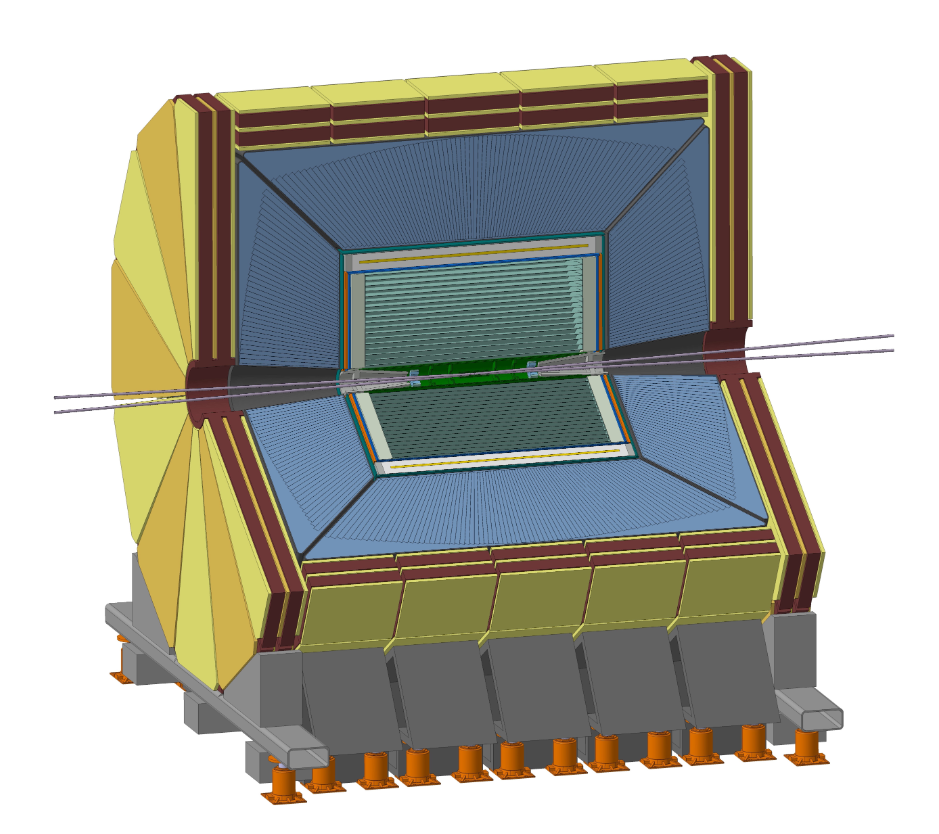
\includegraphics[width=.45\textwidth]{IMG/Cap1/IDEA_art1}} \quad
	\subfloat[][The structure and dimensions of the IDEA detector concept. \label{fig:IDEA_art2}]{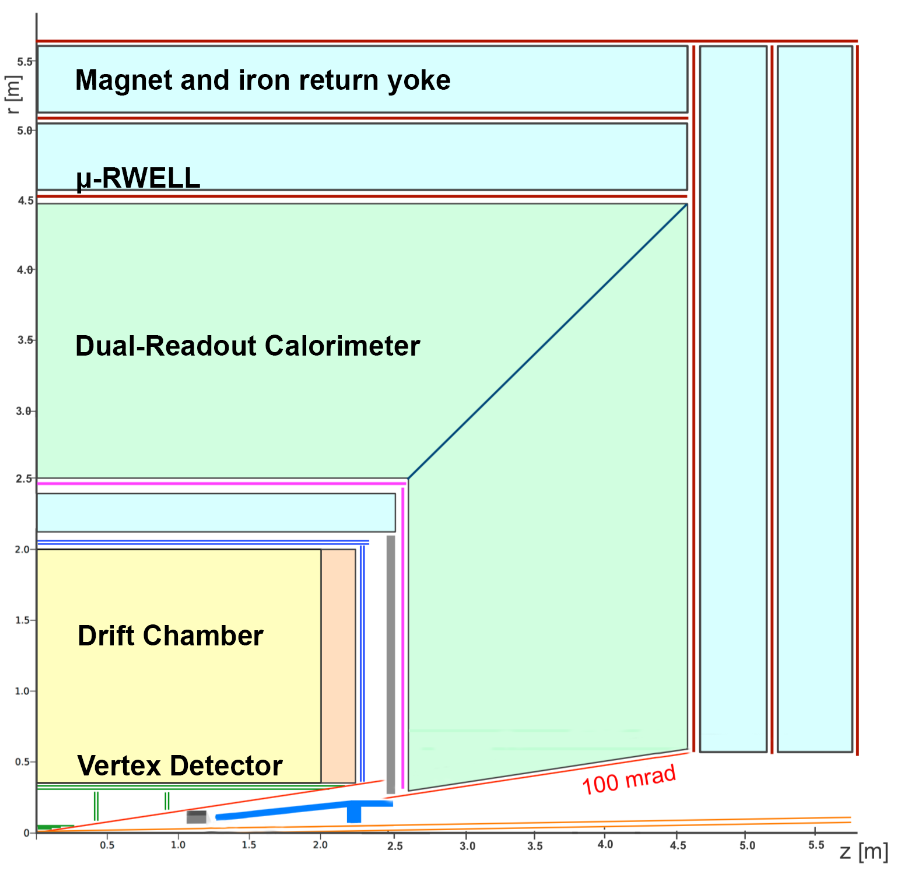
\includegraphics[width=.45\textwidth]{IMG/Cap1/IDEA_art2}}
	\caption{IDEA Detector concept.}
\end{figure}

The IDEA Detector concept is sketched in an artistic view in figure \ref{fig:IDEA_art1} and in its structure and dimensions in figure \ref{fig:IDEA_art2}. 
The overall detector is composed by a silicon pixel vertex detector, a wire chamber surrounded by a layer of silicon micro-strip detectors, a thin superconducting solenoid coil, a pre-shower detector, a dual-readout calorimeter, and muon chambers.
The most innovative elements proposed with this project are:
\begin{itemize}
    \item the ultra-light drift chamber as main tracker;
    \item the Dual-Readout (DR) fiber calorimeter.
\end{itemize}

The drift chamber technology is based on an upgrade of MEG, designed to search for the charged lepton flavor violating decay $\mu \rightarrow e^+\gamma$. The R\&D work studies the construction and operation of the MEG2 Ultra Light TIming Drift Chamber (MULTIDC) performing high momentum resolution and transparency in terms of radiation length.
The IDEA dual-readout calorimeter, on the other hand, stands on the legacy of the DREAM/RD52 Collaboration. The key point is the feasibility of dual-readout optical-fibers calorimeters to obtain high resolution in energy measurement associated to both single-hadron and hadronic jets.
All the most important parameters of the IDEA detector components are listed in table \ref{tab:IDEA_part}.\\
\begin{table}[]
    \centering
    \begin{tabular}{ll}
        \toprule
        Vertex technology                       & Silicon \\
        Vertex inner/outer radius (cm)          & $1.7/34$ \\
        \midrule
        Tracker technology                      & Drift Chamber and Silicon Wrapper\\
        Tracker half length (m)                 & $2.0$ \\
        Tracker outer radius (m)                & $2.0$ \\
        \midrule
        Solenoid field (T)                      & $2.0$ \\
        Solenoid bore radius / half length (m)  & $2.1/30.$ \\
        \midrule
        Preshower absorber                      & Lead \\
        Preshower $R_{min}/R_{max}$ (m)         & $2.4/2.5$ \\
        \midrule
        Calorimeter absorber                    & Copper \\
        Calorimeter $R_{min}/R_{max}$ (m)       & $2.5/4.5$ \\
        \midrule
        Overall height / length (m)             & 11/13 \\
        \bottomrule
    \end{tabular}
    \caption{Parameters of the different sub-detectors composing IDEA.}
    \label{tab:IDEA_part}
\end{table}

\subsection{Vertex detector}
The $1.5\ cm$ beam pipe is surrounded by the IDEA vertex detector composed by pixel active sensors. The structure present high-resistivity substrates architectures implementing on-pixel sparsification and data driven,time stamped readout.
The goal is a thickness of $0.15-0.30\% X_0$ per layer and a power dissipation below $20\ mW/cm^2$.
The vertex detector measures tracks of charged particles with very high precision, of the order of $3\ \mu m$ in the innermost layers, and is able to precisely reconstruct secondary vertices.
This detector will significantly benefit from the electronic and mechanical work for the ALICE ITS \cite{alice_its}, as well as of new ongoing developments, in the framework of the INFN ARCADIA R\&D project.

\subsection{Drift chamber}
The IDEA drift chamber project consist in an ultra-light Drift CHamber (DCH). Following the results obtained by the KLOE Experiment DCH \cite{KLOE} and the recent DCH for MEG2 (the MEG upgrade) \cite{MEG2}, a detector with extraordinary transparency to radiation is designed.\\

The chamber is composed by a unique cylindrical volume, co-axial to the beam axis, with an inner radius of $0.35\ m$ and an outer radius of $2\ m$, for a total length of $4\ m$. It consists of $112$ co-axial layers, at alternating sign stereo angles, grouped in $24$ identical sectors. The ammount of drift cells is $56448$ with variable size from $12.0$ to $14.5\ mm$.
The chamber is operated with a very light gas mixture of $90\%$ He - $10\%$ iC$_4$H$_{10}$ (isobutane), providing a maximum drift value of $\simeq 400\ ns$.\\
The angular coverage extends down to $\simeq 13\deg$, and could be extended with additional silicon disks between the DCH and the calorimeter end caps.\\
In the radial direction the total amount of material is of the order of $1.6\%$ of a radiation length, including inner and outer cylindrical walls and contributions from the gas mixture and the wires. On the other hand, in the forward and backward direction, the total amount of material is equivalent to about $5.0\% X_0$, including inner cylindrical walls and services end plates, instrumented with front-end electronics, signal and HV cables.\\

In the context of the MEG2 drift chamber prototypes \cite{MEG2} with $7\ mm$ cell size, a drift distance resolution of $100\ \mu m$ has been achieved with both a gas mixture and an electrostatic conditions very similar to the ones foreseen for the IDEA DCH.
Analytical calculations assuming this resolution for the DCH allow to study the momentum and angular resolution with the result shown in figure \ref{fig:DCH_res}.
The drift chamber also offers outstanding particle-identification performance using the cluster counting technology improving both spatial resolution and particle identification.

Together with the excellent expected momentum resolution, the DCH can achieve  superior  particle  identification  capabilities  thanks  to  the  cluster-counting  technique. The ionization process for which electrons are released follows a Poison law, therefore by counting the total number of ionization clusters ($N_{cl}$) of a charged track one can reach a relative resolution on $N_{cl}$ that follows $1/\sqrt{N_{cl}}$. The expected performance relative to particle separation in terms of number of standard deviations as a function of the particle momentum are shown in figure \ref{fig:DCH_separation}. In this graph the solid  curves  refer  to  the  cluster-counting  technique,  while  the  dashed  one  refers  to  the expected identification power for the traditional $dE/dx$ method. As it can seen, the particle separation by cluster counting is more performing in the whole range of momentum.

\begin{figure}
	\centering
	\subfloat[][Momentum and angular resolutions for $\theta= 90 \deg$ as a function of momentum. \label{fig:DCH_res}]{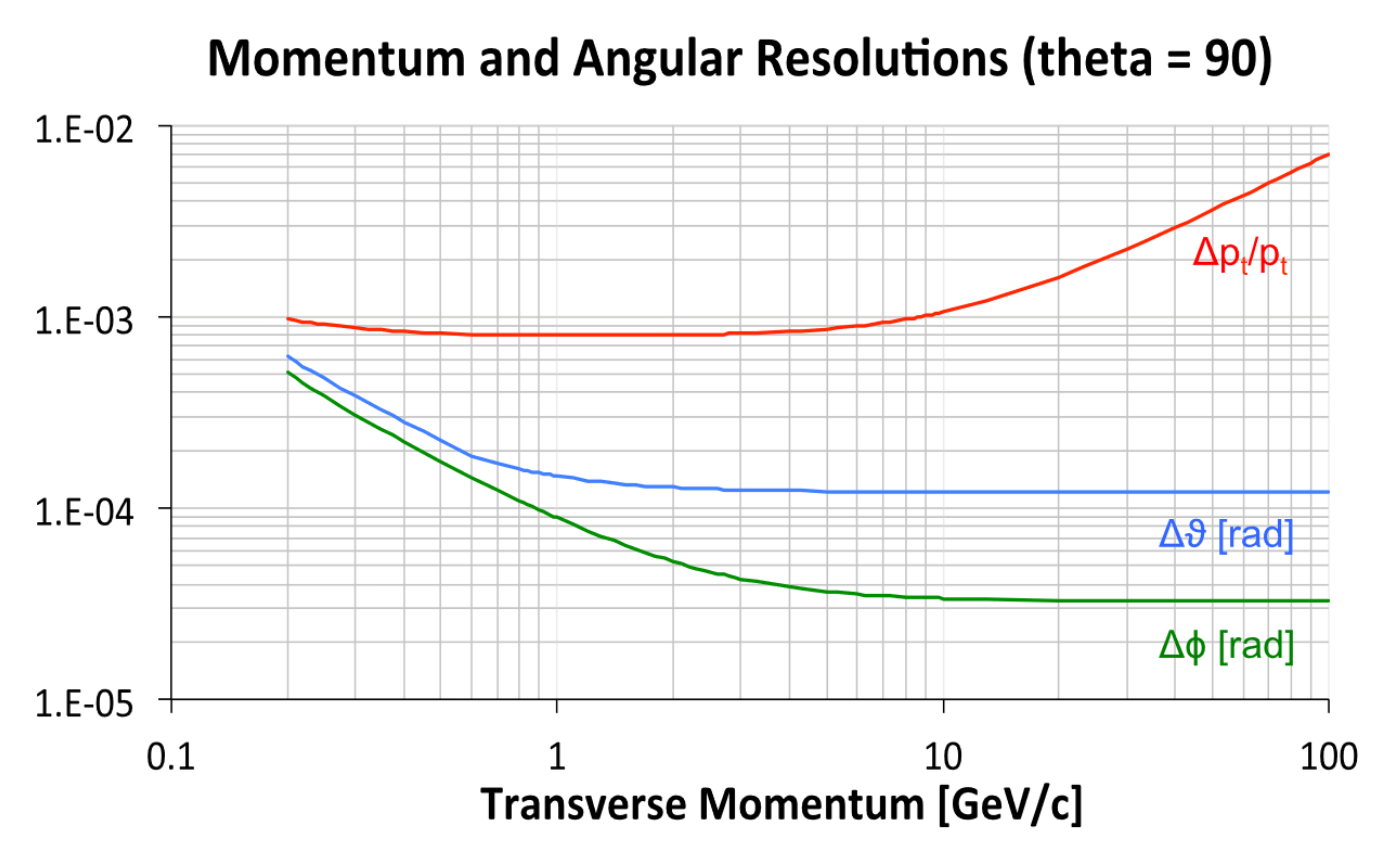
\includegraphics[width=.45\textwidth]{IMG/Cap1/DCH_res.png}} \quad
	\subfloat[][Particle type separation in units of standard deviations as a function of momentum, with cluster counting (solid curves) and with $dE/dx$ (dashed curves). \label{fig:DCH_separation}]{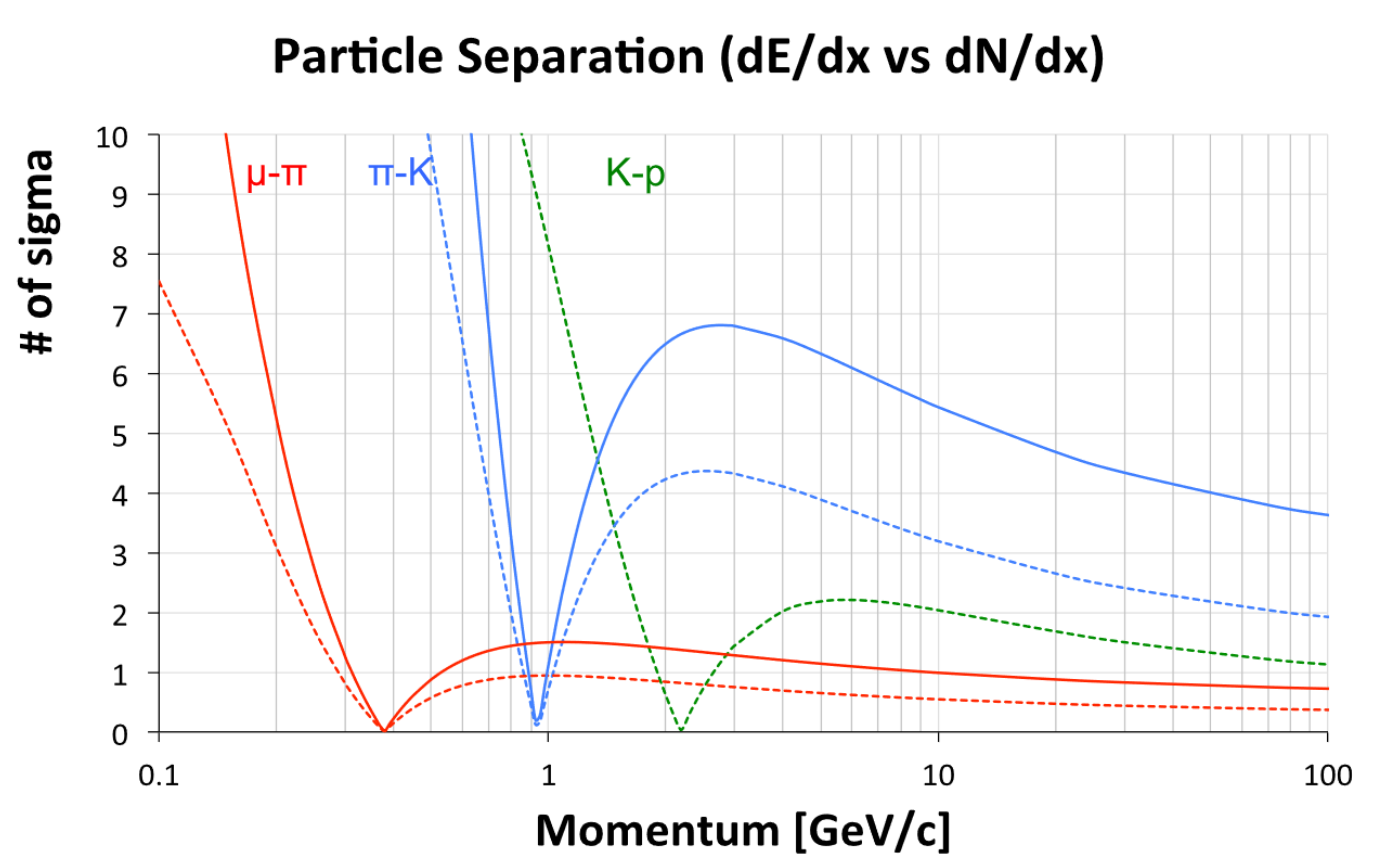
\includegraphics[width=.45\textwidth]{IMG/Cap1/DCH_separation.png}}
	\caption{IDEA ultra-light drift chamber performances \cite{FCC-ee_design}}
\end{figure}

\subsection{Magnet system}
The IDEA detector magnet is an ultra-thin and light (thus “radiation-transparent”) superconducting solenoid. It is $5\ m$ long and has an inner diameter of $4.2\ m$. equipped with a thin iron return yoke. The main feature is that the solenoid is positioned between the tracker block and the calorimeter, a solution currently employed in ATLAS.
This choice impose to keep the total thickness at $30\ cm$ level, below $1 X_0$  in terms of radiation length, but at the same time the stored energy is reduced by a factor four and the cost can be halved.
In this scenario a relatively low field of $2\ T$ can be produced.
The flux return yoke scales with the square of the coil diameter, thus with the given dimensions a yoke thickness of less than $100\ cm$ of iron is sufficient to contain the magnetic flux and to shield the muon chambers.

\subsection{Dual-readout calorimeter}
aaa

\subsection{Preshower and muon chambers}
Both the IDEA preshower and the muon chambers are based on the micro-Resistive WELL($\mu$-RWELL) technology [35]. $\mu$-RWELL chambers are compact Micro-Patter Gaseous Detector (MPGD), with a single amplification stage intrinsically spark protected.\\

A preshower detector is located in the barrel region between the magnet and the calorimeter and another one in the forward region between the drift chamber and the end-cap calorimeter.
In the barrel region, the magnet coil play also the role of of about $1 X_0$ and it is followed by one layer of MPGD chambers; a second layer of chambers follows after another $1 X_0$ of lead. In the forward region an analogue structure is built with both the $\mu$-RWELL layers preceded by $1 X_0$-long lead absorber.\\
The evaluation of the preshower performance and the single-hit-position resolution requirement are still in progress.
But with the now-a-day performances already allow to tag $\simeq 30\%$ of the $\pi^0$ from their $\gamma\gamma$ decay and provides good acceptance for photons.
This technology will perfectly match also the requirements for the IDEA muon system, providing a good tracking efficiency, high-voltage stability, a space resolution for the coordinates of a muon track of $200-300\ \mu m$ and a good time resolution thank to the fast charge amplification process.\\

Also the muon detector uses as well the $\mu$-RWELL technology but with a wider strip pitch, due to the greater dimensions.  It is subdivided in three active layers at increasing distance from the vertex, and located within the iron return yoke that closes the magnetic field. Each MPGD can provide a space point with a spatial resolution of about $400\ \mu m$ in the plane perpendicular to the particle direction. Combining the three stations allows to perform standalone tracking of charged particles at $5-6\ m$ from the vertex. Such a precision also allows to identify secondary vertices that could be produced by long lived particles.